% ===================================================================
%  Supplementary Material for:
%  "Scanner Vendor Harmonization of Spinal Cord Quantitative MRI
%   Biomarkers: A Five-Method Benchmark"
%  Human Brain Mapping
% ===================================================================
\documentclass[12pt,a4paper]{article}
\usepackage[utf8]{inputenc}
\usepackage[T1]{fontenc}
\usepackage[margin=2.5cm]{geometry}
\usepackage{graphicx}
\usepackage{amsmath}
\usepackage{booktabs}
\usepackage{hyperref}
\usepackage{setspace}
\usepackage{enumitem}
\usepackage{float}
\usepackage{multirow}
\usepackage{siunitx}
\usepackage{xurl}
\onehalfspacing

\begin{document}

\section*{Supplementary Material}

\subsection*{S1. Cohort Flow and Missingness}

Of 267 subjects in the spine-generic dataset (release r20231212), 203 were healthy controls (HC) and 64 had pathology (62 mild cervical compression; 2 degenerative cervical myelopathy). Both cohorts were pre-specified prior to analysis.

\textbf{Missingness patterns.} Among HC subjects, 15 (7.4\%) were missing one or more biomarkers: MTR ($n=13$), MTsat ($n=18$), FA/MD/AD/RD ($n=7$ each). Missingness was attributable to acquisition failure or automated QC rejection during pipeline processing (SCT v7.4 QC metrics including PAM50 template overlap, diffusion tensor model-fit residuals, and MT saturation map artifact screening), not to demographic or vendor characteristics. Among ALL subjects, 21 (7.9\%) were incomplete. The complete-case HC cohort comprised $N=188$ and the complete-case ALL cohort $N=246$.

\textbf{Table S1.} Demographic characteristics by vendor (ALL cohort, $N=246$).

\vspace{4mm}
\begin{table}[H]
\centering
\footnotesize
\setlength{\tabcolsep}{2.5pt}
\begin{tabular}{lccccc}
\toprule
\textbf{Characteristic} & \textbf{GE ($n=33$)} & \textbf{Philips ($n=47$)} & \textbf{Siemens ($n=166$)} & \textbf{Total ($n=246$)} & \textbf{$p$} \\
\midrule
Sites ($n$)         & 5 & 8 & 27 & 40 & --- \\
Age (years)         & 28.0 $\pm$ 5.2 & 29.4 $\pm$ 4.7 & 30.0 $\pm$ 6.3 & 29.6 $\pm$ 5.9 & 0.193 \\
Sex (\% female)      & 48.5 & 46.8 & 47.0 & 47.2 & 0.986 \\
Pathology (HC/MC/DCM) & 25/8/0 & 33/13/1 & 130/35/1 & 188/56/2 & 0.661 \\
\bottomrule
\end{tabular}
\end{table}

\subsection*{S2. Biomarker Extraction and Quality Control}

All biomarkers were extracted using the Spinal Cord Toolbox (SCT v7.4; \url{https://spinalcordtoolbox.com}) following the spine-generic processing pipeline documentation (\url{https://spine-generic.readthedocs.io}).

\textbf{Processing steps:}
\begin{itemize}[nosep]
  \item \textbf{C2--C3 level identification:} Automated PAM50 template registration.
  \item \textbf{CSA:} Deep-learning segmentation (\texttt{sct\_deepseg\_sc}) on T2w images.
  \item \textbf{GM-CSA:} Gray matter segmentation via \texttt{sct\_deepseg\_gm} (T2*-weighted contrast).
  \item \textbf{MTR/MTsat:} Computed from MT-on and MT-off acquisitions.
  \item \textbf{DTI metrics:} Diffusion tensor fitting via \texttt{sct\_dmri\_compute\_dti}.
\end{itemize}

\textbf{QC rejection criteria:} Segmentation overlap with PAM50 template $<0.6$; DTI model-fit residual $>2$ SD above cohort mean; MT saturation map visual artifact flag.

\subsection*{S3. Harmonization Methods: Mathematical Details}

\textbf{S3.1 ComBat (per-metric).} For each biomarker $y_{ijv}$ for subject $i$ at site $v$:
\begin{equation*}
y_{ijv}^{\text{harm}} = \frac{y_{ijv} - \hat{\alpha}_v - X_{ij}\hat{\beta}}{\hat{\gamma}_v} + X_{ij}\hat{\beta}
\end{equation*}
where $\hat{\alpha}_v$ and $\hat{\gamma}_v$ are vendor-specific location and scale parameters estimated with empirical Bayes shrinkage, and $X_{ij}$ is the design matrix of biological covariates (age, sex). This is the standard ComBat formulation [8,9] applied independently to each biomarker.

\textbf{S3.2 ComBat-joint.} All eight biomarkers are modeled jointly with a shared vendor parameter estimated via joint empirical Bayes (\texttt{eb=True} in neuroCombat). The mathematical form is identical to S3.1 but $\hat{\alpha}_v$ and $\hat{\gamma}_v$ are estimated simultaneously across biomarkers, preserving cross-metric covariance structure.

\textbf{S3.3 CovBat.} After ComBat-joint harmonization, the residual matrix $E$ (subjects $\times$ biomarkers) is decomposed via PCA: $E = ZW^T$, where $Z$ is the PC score matrix and $W$ is the loading matrix. PCs explaining at least 95\% of the residual variance were retained ($K=5$ of 8 in both cohorts; see Supplementary Fig.~S4 for the resulting covariance structure). Each PC $k$ is then harmonized independently: $Z_{k}^{\text{harm}} = (Z_k - \hat{\alpha}_{vk})/\hat{\gamma}_{vk}$, where $\hat{\alpha}_{vk}$ and $\hat{\gamma}_{vk}$ are vendor-specific parameters for PC $k$. The harmonized data are reconstructed as $Y^{\text{harm}} = Y^{\text{ComBat-joint}} + Z^{\text{harm}}W^T$.

\textbf{S3.4 RELIEF.} After ComBat-joint harmonization, residuals undergo ICA decomposition: $E = SA^T$, where $S$ is the independent component score matrix and $A$ is the mixing matrix. For each component $c$, a one-way ANOVA tests vendor association. Components with Benjamini-Hochberg FDR-controlled $q < 0.05$ are zeroed ($S_c \leftarrow 0$). The remaining components are recombined: $E^{\text{RELIEF}} = S^{\text{cleaned}}A^T$.

\textbf{S3.5 LME/FE.} For each biomarker:
\begin{equation*}
y_{ijv} = \beta_0 + \beta_1 \text{Age}_i + \beta_2 \text{Sex}_i + u_v + \varepsilon_{ijv}
\end{equation*}
where $u_v \sim \mathcal{N}(0, \sigma_u^2)$ is the vendor-specific random intercept. Harmonized values: $y_{ijv}^{\text{harm}} = y_{ijv} - \hat{u}_v$ when LME converges; $y_{ijv}^{\text{harm}} = y_{ijv} - \bar{y}_v + \bar{y}$ (OLS centering) when the random-effects covariance matrix is singular (FE fallback).

\subsection*{S4. Evaluation Metrics: Computational Details}

\textbf{S4.1 Vendor $\eta^2$.} One-way ANOVA: $\eta^2 = \text{SS}_{\text{vendor}} / \text{SS}_{\text{total}}$. Reported as mean across 8 biomarkers.

\textbf{S4.2 PERMANOVA.} Euclidean distance matrix on the 8-dimensional biomarker space after per-dimension z-scoring. 9,999 permutations of vendor labels. $R^2 = \text{SS}_{\text{vendor}} / \text{SS}_{\text{total}}$ from the distance-based pseudo-$F$ statistic [20]. Implementation: custom NumPy code (pseudo-$F$ and permutation loop written in-house; no third-party PERMANOVA package). On z-scored features with Euclidean distance, the multivariate $R^2$ equals the mean of the per-dimension $\eta^2$ computed on the same subjects. Because all five methods and the unharmonised baseline are fitted and evaluated on the same unified complete-case sample (HC $N=188$, ALL $N=246$), this identity holds exactly for every method, so univariate and multivariate summaries are directly comparable.

\textbf{S4.3 Biological $R^2$.} Type-II semi-partial $R^2$ from linear models: $\text{biomarker} \sim \text{Age} + \text{Sex}$. Reported as mean across biomarkers.

\textbf{S4.4 Subject-level preservation.} Pearson correlation between pre- and post-harmonization 8-dimensional biomarker vectors, computed per subject and averaged:
\[ r = \text{mean}_i[\text{corr}(y_i^{\text{pre}}, y_i^{\text{post}})]. \]

\textbf{S4.5 Unified complete-case analysis sample.} All results in the main text and this supplement are computed on a single pre-specified complete-case sample per cohort: HC $N=188$ and ALL $N=246$ (all eight biomarkers plus age, sex, and vendor observed). ComBat and LME/FE were refitted on this unified sample (the ComBat and LME/FE columns of every table therefore derive from these refits); ComBat-joint, CovBat, and RELIEF are complete-case by construction because they require the full joint biomarker panel. This unified definition replaces the earlier per-metric maximum-available-sample evaluation and removes any sample mismatch between univariate and multivariate endpoints.

\textbf{S4.6 Within-resample paired bootstrap.} To compare $r_{\text{pre,post}}$ between method pairs, each stratified bootstrap resample ($B=2{,}000$, resampling subjects within vendor strata) was passed to \emph{all} methods simultaneously; the per-resample differences $r_A - r_B$ form the null distribution for the pairwise test. This pairing removes between-resample variance (the source of the overlapping marginal CIs) and directly targets the pairwise contrast. Results: in HC, 8 of 10 method pairs were significantly separated (all $p\leq0.003$; ComBat vs.\ CovBat $p=0.070$ and ComBat vs.\ RELIEF $p=0.694$ were not); in ALL, 9 of 10 pairs were separated (ComBat vs.\ RELIEF $p=0.403$ was not). LME/FE was significantly highest and CovBat significantly lowest in both cohorts. Full results in Supplementary Table~S7.

\textbf{Table S7.} Within-resample paired bootstrap comparison of subject-level preservation ($r_{\text{pre,post}}$) between all method pairs ($B=2{,}000$, stratified by vendor; complete-case sample). $\Delta r = r_A - r_B$; CI = 95\% percentile interval of the per-resample differences; $p$ = two-sided bootstrap p-value. HC cohort above, ALL cohort below.

\vspace{4mm}
\begin{table}[H]
\centering
\begin{tabular}{llcccl}
\toprule
\textbf{Cohort} & \textbf{Comparison} & {$\Delta r$} & \textbf{95\% CI} & {$p$} & \textbf{Significant} \\
\midrule
\multirow{10}{*}{HC}
  & ComBat vs.\ ComBat-joint & $-$0.017 & [$-$0.020, $-$0.014] & 0.0005 & Yes \\
  & ComBat vs.\ CovBat & 0.007 & [$-$0.000, 0.015] & 0.070 & No \\
  & ComBat vs.\ RELIEF & $-$0.001 & [$-$0.007, 0.005] & 0.694 & No \\
  & ComBat vs.\ LME/FE & $-$0.027 & [$-$0.033, $-$0.020] & 0.0005 & Yes \\
  & ComBat-joint vs.\ CovBat & 0.024 & [0.017, 0.032] & 0.0005 & Yes \\
  & ComBat-joint vs.\ RELIEF & 0.016 & [0.010, 0.022] & 0.0005 & Yes \\
  & ComBat-joint vs.\ LME/FE & $-$0.010 & [$-$0.015, $-$0.004] & 0.003 & Yes \\
  & CovBat vs.\ RELIEF & $-$0.009 & [$-$0.015, $-$0.003] & 0.002 & Yes \\
  & CovBat vs.\ LME/FE & $-$0.034 & [$-$0.043, $-$0.025] & 0.0005 & Yes \\
  & RELIEF vs.\ LME/FE & $-$0.026 & [$-$0.033, $-$0.018] & 0.0005 & Yes \\
\midrule
\multirow{10}{*}{ALL}
  & ComBat vs.\ ComBat-joint & $-$0.013 & [$-$0.015, $-$0.011] & 0.0005 & Yes \\
  & ComBat vs.\ CovBat & 0.011 & [0.005, 0.018] & 0.001 & Yes \\
  & ComBat vs.\ RELIEF & 0.002 & [$-$0.003, 0.008] & 0.403 & No \\
  & ComBat vs.\ LME/FE & $-$0.027 & [$-$0.033, $-$0.020] & 0.0005 & Yes \\
  & ComBat-joint vs.\ CovBat & 0.024 & [0.018, 0.031] & 0.0005 & Yes \\
  & ComBat-joint vs.\ RELIEF & 0.015 & [0.010, 0.020] & 0.0005 & Yes \\
  & ComBat-joint vs.\ LME/FE & $-$0.014 & [$-$0.019, $-$0.008] & 0.0005 & Yes \\
  & CovBat vs.\ RELIEF & $-$0.009 & [$-$0.015, $-$0.004] & 0.001 & Yes \\
  & CovBat vs.\ LME/FE & $-$0.038 & [$-$0.046, $-$0.029] & 0.0005 & Yes \\
  & RELIEF vs.\ LME/FE & $-$0.029 & [$-$0.035, $-$0.022] & 0.0005 & Yes \\
\bottomrule
\end{tabular}
\end{table}

\subsection*{S5. LOVO External Validation: Protocol}

\textbf{Training.} For each method, harmonization models were fitted on subjects from two vendors (training set). The third vendor was entirely held out as test set.

\textbf{Transformation of unseen vendors:}
\begin{itemize}[nosep]
  \item \textbf{ComBat/ComBat-joint:} Test-vendor biomarker values were z-scored to the training-vendor harmonized distribution: $y_{\text{test}}^{\text{harm}} = (y_{\text{test}} - \mu_{\text{test}}) \times (\sigma_{\text{train}}^{\text{harm}} / \sigma_{\text{test}}) + \mu_{\text{train}}^{\text{harm}}$.
  \item \textbf{CovBat:} Test-vendor residuals were projected onto training PCA space; PC scores were z-score matched to training PC-score distribution.
  \item \textbf{RELIEF:} Test-vendor residuals were projected onto training ICA space via $\text{inv}(A^T)$; batch-flagged components were zeroed using the training-vendor flag set.
  \item \textbf{LME/FE:} Test-vendor offset set to 0; test-vendor values were carried through essentially untransformed (raw values, no vendor or covariate adjustment).
\end{itemize}

\textbf{Evaluation.} The same three endpoints were computed after pooling the harmonised training-vendor and held-out test-vendor data within each fold, then averaged across the 3 rotation folds. Because the transformation applied to the test vendor is per-biomarker affine (location--scale) for ComBat, ComBat-joint, and LME/FE, the test-vendor pre/post correlation equals 1.0 by construction for these methods; their preservation statistics therefore reflect the pooled sample rather than the unseen vendor in isolation. Similarly, the LOVO/internal $\eta^2$ ratio below 1 for ComBat-joint reflects the pooled evaluation sample rather than genuine improvement on unseen vendors. For CovBat and RELIEF, projection onto the training PCA/ICA basis mixes biomarker dimensions, and the test-vendor pre/post correlation fell below 1 ($r=0.85$--$0.97$ across folds), providing a genuine held-out-vendor distortion measure (Table~S6).

\textbf{Table S6.} Test-vendor-only evaluation metrics by held-out vendor and method (mean across 8 biomarkers; complete-case training sample $N=188$). |shift|: mean absolute shift of the held-out-vendor mean relative to the pooled training distribution, in training-SD units; var ratio: held-out-vendor to training variance ratio; centroid shift: multivariate centroid shift in pooled SD units; $r_{\text{pre,post}}$: test-vendor pre/post correlation. ComBat and ComBat-joint force the test-vendor distribution onto the training template (shift exactly 0 by construction); CovBat leaves small residual shifts; RELIEF and LME/FE leave the held-out vendor shifted relative to training.

\vspace{4mm}
\begin{table}[H]
\centering
\begin{tabular}{llSSSl}
\toprule
\textbf{Held-out} & \textbf{Method} & {$|\text{shift}|$} & \textbf{var ratio} & \textbf{centroid shift} & \textbf{$r_{\text{pre,post}}$ (test)} \\
\midrule
\multirow{6}{*}{GE} 
  & Original & 1.46 & 0.98 & 5.68 & 1.000 \\
  & ComBat & 0.00 & 1.00 & 0.00 & 1.000 \\
  & ComBat-joint & 0.00 & 1.00 & 0.00 & 1.000 \\
  & CovBat & 0.03 & 0.94 & 0.12 & 0.851 \\
  & RELIEF & 1.64 & 1.12 & 5.97 & 0.925 \\
  & LME/FE & 1.62 & 1.08 & 5.92 & 1.000 \\
\midrule
\multirow{6}{*}{Philips} 
  & Original & 0.80 & 0.83 & 2.58 & 1.000 \\
  & ComBat & 0.00 & 1.00 & 0.00 & 1.000 \\
  & ComBat-joint & 0.00 & 1.00 & 0.00 & 1.000 \\
  & CovBat & 0.03 & 1.00 & 0.10 & 0.949 \\
  & RELIEF & 0.85 & 0.97 & 2.69 & 0.973 \\
  & LME/FE & 0.92 & 0.99 & 3.14 & 1.000 \\
\midrule
\multirow{6}{*}{Siemens} 
  & Original & 1.05 & 0.93 & 3.37 & 1.000 \\
  & ComBat & 0.00 & 1.00 & 0.00 & 1.000 \\
  & ComBat-joint & 0.00 & 1.00 & 0.00 & 1.000 \\
  & CovBat & 0.05 & 0.96 & 0.16 & 0.911 \\
  & RELIEF & 1.42 & 1.24 & 4.54 & 0.960 \\
  & LME/FE & 1.39 & 1.13 & 4.51 & 1.000 \\
\bottomrule
\end{tabular}
\end{table}

\subsection*{S6. Design C Balanced-Subsample Analysis}

To isolate the effect of vendor imbalance, Siemens was randomly subsampled to 40 subjects per seed (HC cohort, retaining all GE and Philips subjects), yielding subsets of approximately 98 subjects with a more balanced vendor composition (GE 25, Philips 33, Siemens 40). For each of 20 random seeds, all five harmonisation methods were refitted on the subset using the same canonical implementations as the main analysis, and vendor $\eta^2$, PERMANOVA $R^2$, subject-level preservation ($r_{\text{pre,post}}$), and age-signal recovery were recomputed. Results are shown in Supplementary Fig.~S2.

\subsection*{S7. Supplementary Figures}

\begin{figure}[H]
\centering
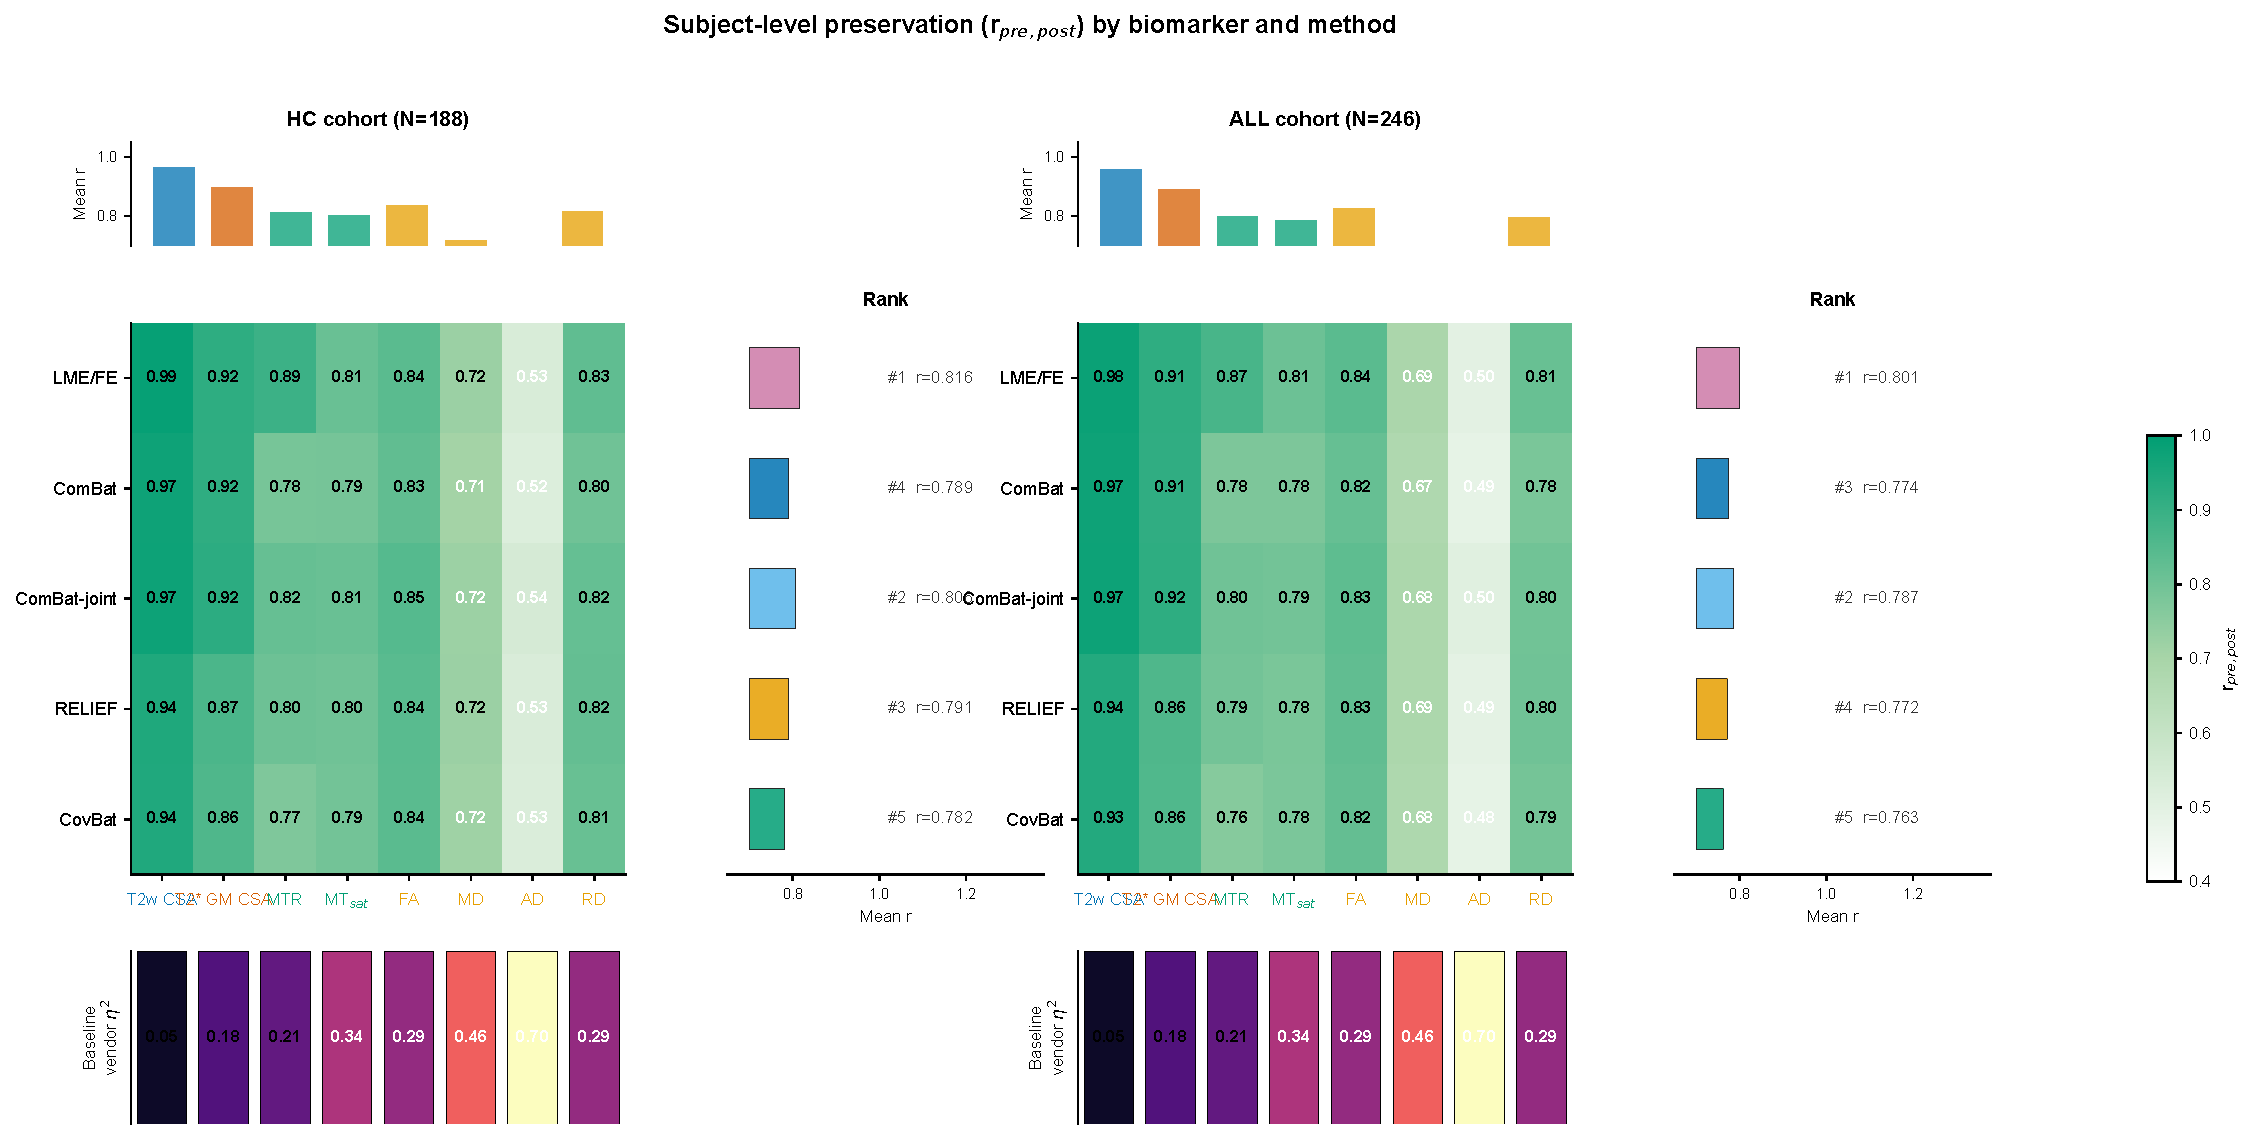
\includegraphics[width=0.85\textwidth]{FigS1_rpre_post.pdf}
\caption{Subject-level preservation ($r_{\text{pre,post}}$) by method. Marginal distributions of per-subject Pearson correlations between pre- and post-harmonization 8-dimensional biomarker vectors. Higher values indicate better preservation of subject ranking. LME/FE shows highest preservation ($r=0.82$); CovBat lowest ($r=0.78$).}
\end{figure}

\begin{figure}[H]
\centering
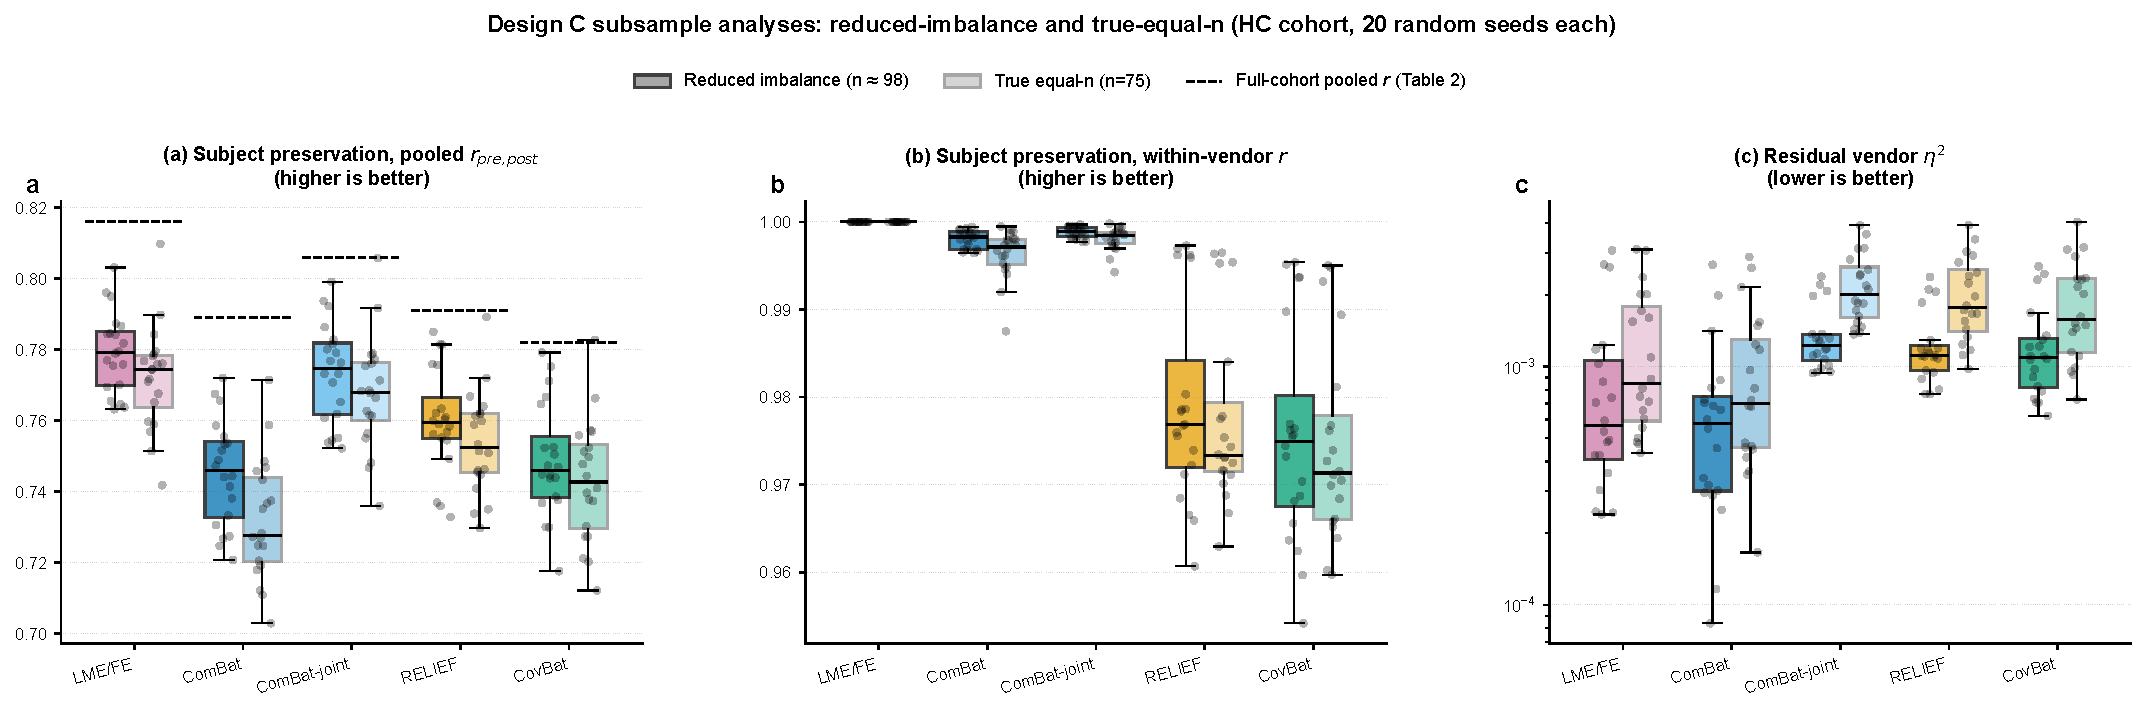
\includegraphics[width=0.85\textwidth]{FigS2_designC.pdf}
\caption{Design C balanced-subsample robustness analysis. (a) $r_{\text{pre,post}}$ distributions across 20 random subsampling seeds (Siemens restricted to 40 subjects per seed, all GE and Philips subjects retained; $n\approx98$ per subset; HC cohort). (b) Vendor effect ($\eta^2$) distributions on logarithmic scale; the dashed line marks the unharmonised baseline ($\eta^2=0.374$). Under balanced conditions the preservation hierarchy reversed: ComBat-family methods converged to near-perfect preservation ($r=0.99$--$1.00$; CovBat $0.991$, others $\geq0.998$) while LME/FE remained at $r=0.843$. The main-analysis preservation gradient therefore largely reflects real-world vendor imbalance (Siemens 166/246, 67\%) rather than intrinsic method limitations.}
\end{figure}

\begin{figure}[H]
\centering
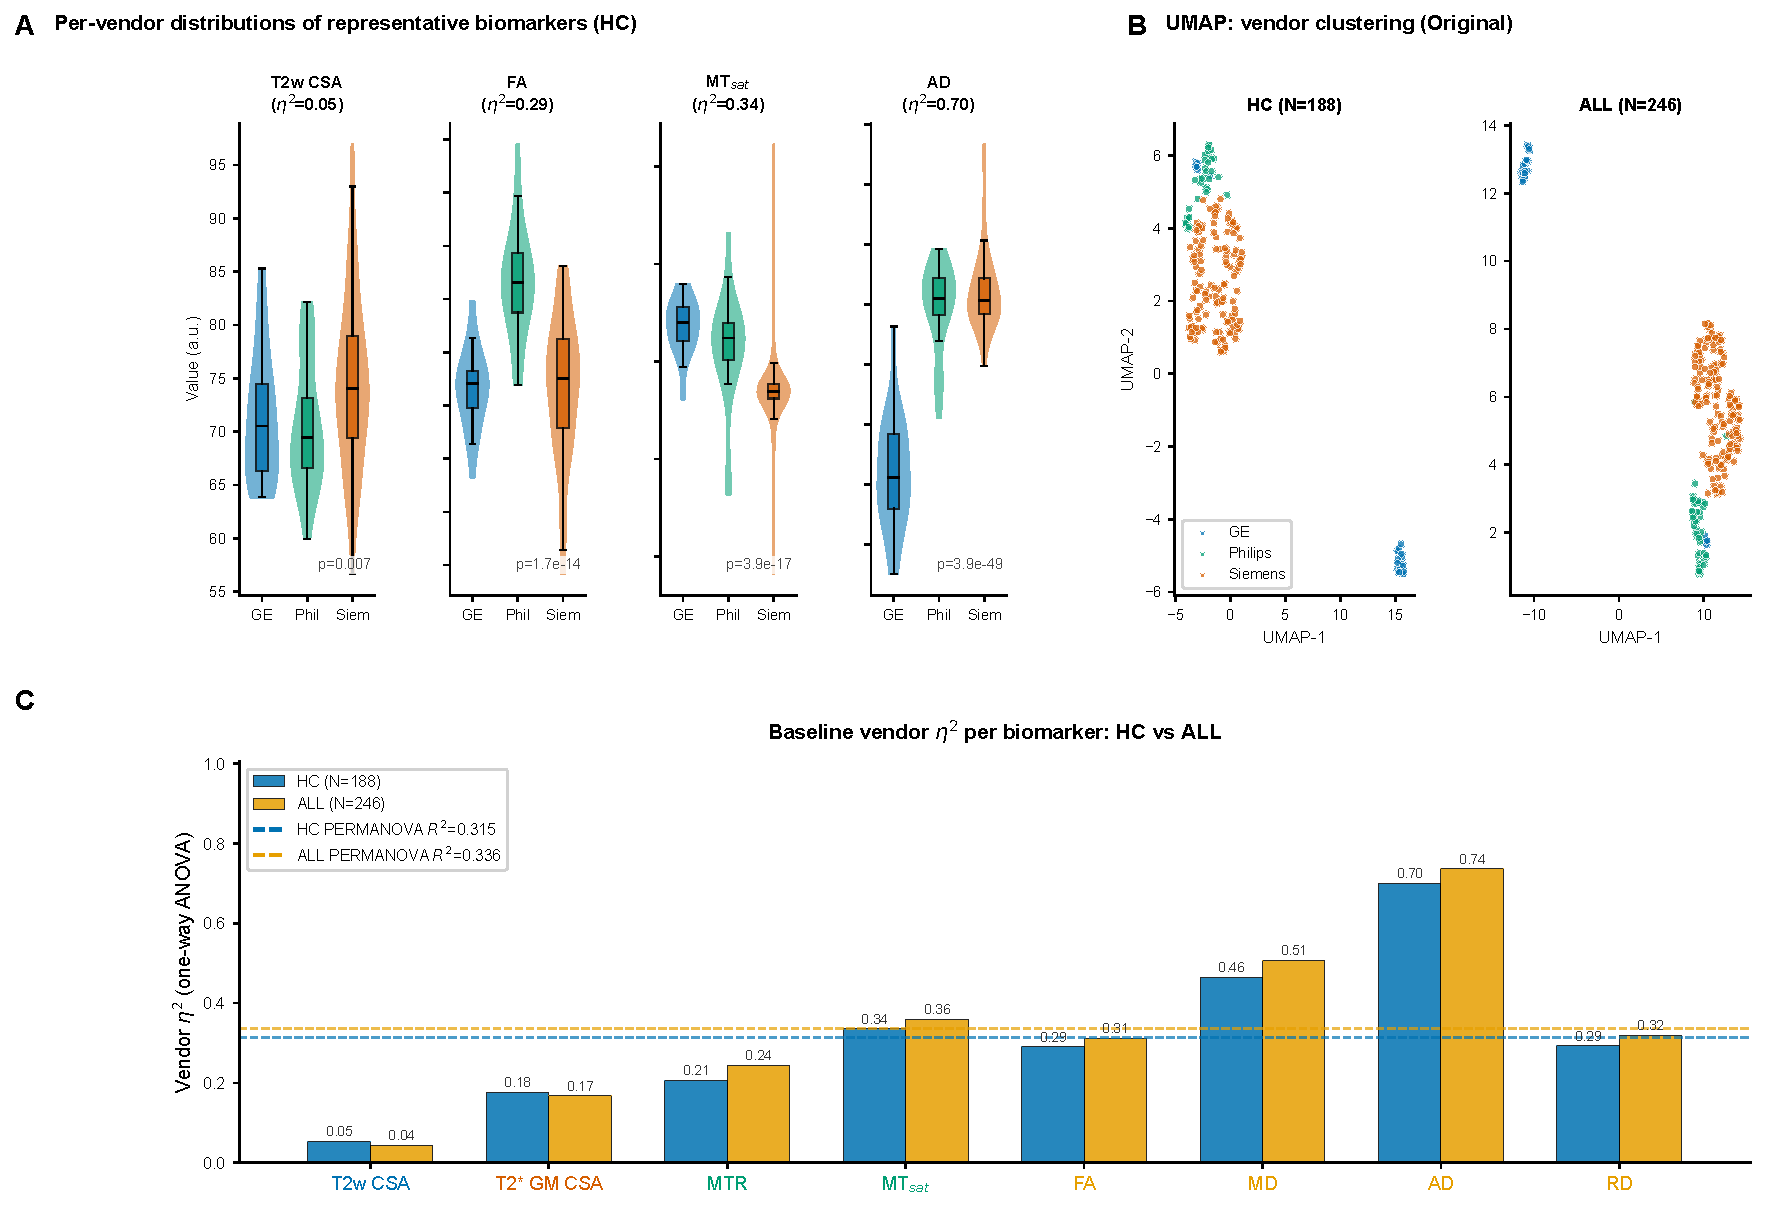
\includegraphics[width=0.85\textwidth]{FigS3_baseline.pdf}
\caption{Baseline vendor effects in spinal cord qMRI biomarkers. \textbf{(a)} Per-vendor distributions of four representative biomarkers in the HC cohort (T2w-CSA $\eta^2=0.05$; FA $0.29$; MTsat $0.34$; AD $0.70$; one-way ANOVA $p$ values shown). \textbf{(b)} UMAP embedding of the 8-dimensional biomarker space (Original, unharmonised data) coloured by vendor, for the HC ($N=188$) and ALL ($N=246$) cohorts. \textbf{(c)} Per-biomarker baseline vendor $\eta^2$ in the HC and ALL cohorts; mean $\eta^2=0.31$ (HC) and $0.34$ (ALL); PERMANOVA $R^2=0.315$ (HC) and $0.336$ (ALL), both $p=1\times10^{-4}$ (permutation lower bound with 9,999 permutations).}
\end{figure}

\begin{figure}[H]
\centering

\includegraphics[width=0.85\textwidth]{FigS4_covariance.pdf}
\caption{Cross-metric covariance structure preservation. \textbf{(a)} Pearson correlation matrices of the eight biomarkers (HC cohort, $N=188$) before and after each method. \textbf{(b)} Frobenius distance between the correlation matrices of each pair of methods (lower = more similar covariance structure). CovBat and RELIEF are the closest (HC: 0.09, ALL: 0.08), indicating near-identical covariance structure despite the additional ICA round-trip in RELIEF. ComBat-joint and ComBat are also close (HC: 0.05, ALL: 0.04), showing that joint empirical Bayes has limited impact on the covariance structure beyond the per-metric ComBat baseline. ComBat (HC: 1.55, ALL: 1.64) and LME/FE (HC: 1.56, ALL: 1.65) remain closest to the original, reflecting minimal covariance distortion.}
\end{figure}

\textbf{Table S8.} Per-vendor one-vs-rest AUC (ALL cohort, $N=246$) after fold-internal harmonisation. Hanley--McNeil 95\% CI based on the point estimate; vendor labels are known to the harmonisation step (training and test) but the random forest is blind to them.

\vspace{4mm}
\begin{table}[H]
\centering
\footnotesize
\setlength{\tabcolsep}{3pt}
\begin{tabular}{lcccccc}
\toprule
\textbf{Method} & \textbf{GE AUC} & \textbf{95\% CI} & \textbf{Philips AUC} & \textbf{95\% CI} & \textbf{Siemens AUC} & \textbf{95\% CI} \\
\midrule
Original      & 0.980 & [0.947, 1.014] & 0.987 & [0.964, 1.010] & 0.993 & [0.984, 1.002] \\
ComBat        & 0.803 & [0.709, 0.896] & 0.666 & [0.575, 0.758] & 0.722 & [0.658, 0.786] \\
ComBat-joint  & 0.766 & [0.668, 0.865] & 0.669 & [0.578, 0.761] & 0.729 & [0.666, 0.792] \\
CovBat        & 0.585 & [0.476, 0.693] & 0.698 & [0.609, 0.788] & 0.669 & [0.600, 0.738] \\
RELIEF        & 0.725 & [0.622, 0.828] & 0.691 & [0.601, 0.781] & 0.738 & [0.676, 0.800] \\
LME/FE        & 0.907 & [0.838, 0.977] & 0.722 & [0.634, 0.810] & 0.849 & [0.802, 0.895] \\
\bottomrule
\end{tabular}
\end{table}

\subsection*{S8. Supplementary Data}

The following data files are provided:
\begin{itemize}[nosep]
  \item \texttt{biomarkers\_master.csv}: Raw biomarker values with demographics (267 subjects)
  \item \texttt{demographics\_completecase.csv}: Complete-case analysis sample demographics by vendor and cohort (Supplementary Table~S1)
  \item \texttt{lovo\_summary.csv}: Leave-one-vendor-out validation results (18 rows)
  \item \texttt{lovo\_testvendor.csv}: Leave-one-vendor-out held-out (test) vendor shifts and correlations per fold, method, and biomarker (162 rows; Supplementary Table~S6)
  \item \texttt{corr\_matrices\_HC.csv} / \texttt{corr\_matrices\_ALL.csv}: Full 8$\times$8 Pearson correlation matrices for all six methods (Supplementary Fig.~S4)
  \item \texttt{frobenius\_distance\_HC.csv} / \texttt{frobenius\_distance\_ALL.csv}: Pairwise Frobenius distances between method correlation matrices (Supplementary Fig.~S4)
  \item \texttt{comparison\_long.csv}: Per-biomarker evaluation metrics (vendor $\eta^2$, age $R^2$, sex $R^2$, $r_{\text{pre,post}}$) for all methods and both cohorts on the unified complete-case sample (96 rows)
  \item \texttt{cc\_summary.csv}: Method-level summary (mean/median/min/max) of the per-biomarker metrics in \texttt{comparison\_long.csv}
  \item \texttt{permanova\_results.csv}: PERMANOVA results (HC and ALL cohorts)
  \item \texttt{bootstrap\_r\_ci\_cc.csv} / \texttt{bootstrap\_eta2\_baseline\_cc.csv}: Bootstrap 95\% confidence intervals for $r_{\text{pre,post}}$ and baseline $\eta^2$ ($B=2{,}000$, stratified by vendor)
  \item \texttt{bootstrap\_paired\_r.csv}: Paired bootstrap tests of $r_{\text{pre,post}}$ differences between method pairs (20 rows; Supplementary Table~S7)
  \item \texttt{lme\_effect\_summary.csv}: LME convergence status per biomarker$\times$cohort
  \item \texttt{relief\_components\_HC.csv} / \texttt{relief\_components\_ALL.csv}: RELIEF ICA component statistics
  \item \texttt{ml\_leakfree\_summary.csv}: Fold-internal machine-learnability summary (vendor, pathology, and sex AUC by method and cohort)
  \item \texttt{ml\_leakfree\_vendorclass.csv}: Per-vendor one-vs-rest AUC after fold-internal harmonisation (Supplementary Table~S8)
  \item \texttt{ml\_leakfree\_paired.csv}: Paired comparison of pathology AUC (Original vs each method, within-resample)
  \item \texttt{lovo\_permanova\_z.csv}: Z-scored PERMANOVA results for the LOVO pooled evaluation sample
\end{itemize}

The analysis code is available at \url{https://github.com/wudengke2010/spine-generic-harmonization}.

\end{document}
